% !TEX program = xelatex

\documentclass[notitlepage,lecture,print]{report}

\usepackage[UTF8]{ctex}
\usepackage{graphicx}

%%%%%%%%%%%%%%%%%%%%%%%%%%%%%%%%%%%%%%%%%%%%%%%%%%%%%%%%%%%%%%%%%%%
% 西文字体:Monaco
% 中文字体:文泉驿微米黑
%%%%%%%%%%%%%%%%%%%%%%%%%%%%%%%%%%%%%%%%%%%%%%%%%%%%%%%%%%%%%%%%%%%
\usepackage{fontspec}
\setmainfont{Monaco}
\setsansfont{Monaco}
\setmonofont{Monaco}
\setCJKmainfont{WenQuanYi Micro Hei}

%%%%%%%%%%%%%%%%%%%%%%%%%%%%%%%%%%%%%%%%%%%%%%%%%%%%%%%%%%%%%%%%%%%
% 添加顔色:solarized light
%%%%%%%%%%%%%%%%%%%%%%%%%%%%%%%%%%%%%%%%%%%%%%%%%%%%%%%%%%%%%%%%%%%
\usepackage{xcolor-solarized}
\usepackage{xcolor}

%%%%%%%%%%%%%%%%%%%%%%%%%%%%%%%%%%%%%%%%%%%%%%%%%%%%%%%%%%%%%%%%%%%
% 页边距
%%%%%%%%%%%%%%%%%%%%%%%%%%%%%%%%%%%%%%%%%%%%%%%%%%%%%%%%%%%%%%%%%%%
\usepackage{geometry}
\geometry{top=15mm,bottom=15mm,left=15mm,right=15mm}

%%%%%%%%%%%%%%%%%%%%%%%%%%%%%%%%%%%%%%%%%%%%%%%%%%%%%%%%%%%%%%%%%%%
% 页眉页脚
%%%%%%%%%%%%%%%%%%%%%%%%%%%%%%%%%%%%%%%%%%%%%%%%%%%%%%%%%%%%%%%%%%%
\usepackage{titleps}
\newpagestyle{main}[\small\bfseries]{
    \sethead
    [][\href{https://github.com/XiMen-classroom}{\color{gray} \large \texttt{XiMen-classroom}}][] % 偶数页
    {}{\href{https://github.com/XiMen-classroom}{\color{gray} \large \texttt{XiMen-classroom}}}{} % 奇数页
    \headrule % 页眉画线
    \setfoot
    {}{-\quad\thepage\quad-}{} % 页脚奇偶页相同
    \footrule % 页脚画线
}
\pagestyle{main}

%%%%%%%%%%%%%%%%%%%%%%%%%%%%%%%%%%%%%%%%%%%%%%%%%%%%%%%%%%%%%%%%%%%
% 脚注样式
%%%%%%%%%%%%%%%%%%%%%%%%%%%%%%%%%%%%%%%%%%%%%%%%%%%%%%%%%%%%%%%%%%%
\usepackage{pifont}
\renewcommand{\thefootnote}{\ding{\numexpr171+\value{footnote}}}
\renewcommand{\thempfootnote}{\fnsymbol{mpfootnote}}

%%%%%%%%%%%%%%%%%%%%%%%%%%%%%%%%%%%%%%%%%%%%%%%%%%%%%%%%%%%%%%%%%%%
% 附录
%%%%%%%%%%%%%%%%%%%%%%%%%%%%%%%%%%%%%%%%%%%%%%%%%%%%%%%%%%%%%%%%%%%
\usepackage[toc,page]{appendix}

%%%%%%%%%%%%%%%%%%%%%%%%%%%%%%%%%%%%%%%%%%%%%%%%%%%%%%%%%%%%%%%%%%%
% 缩小列表环境的行间距
%%%%%%%%%%%%%%%%%%%%%%%%%%%%%%%%%%%%%%%%%%%%%%%%%%%%%%%%%%%%%%%%%%%
\usepackage{enumitem}
\setlist{nolistsep}

%%%%%%%%%%%%%%%%%%%%%%%%%%%%%%%%%%%%%%%%%%%%%%%%%%%%%%%%%%%%%%%%%%%
% 定义 \NOTE 命令
%%%%%%%%%%%%%%%%%%%%%%%%%%%%%%%%%%%%%%%%%%%%%%%%%%%%%%%%%%%%%%%%%%%
\newenvironment{inner_note}[1][.88]
{
    \begin{minipage}{#1\textwidth}
        \colorbox{teal}{\textcolor{yellow}{NOTE}}\\% 提示标题顔色:茶绿背景,黄色字体
}
{
    \end{minipage}
}

\newcommand{\NOTE}[2][.88]{
    \begin{center}
        \fbox{
            \begin{inner_note}[#1]
                #2
            \end{inner_note}
        }
    \end{center}
}

%%%%%%%%%%%%%%%%%%%%%%%%%%%%%%%%%%%%%%%%%%%%%%%%%%%%%%%%%%%%%%%%%%%
% 带缩进的列表
%%%%%%%%%%%%%%%%%%%%%%%%%%%%%%%%%%%%%%%%%%%%%%%%%%%%%%%%%%%%%%%%%%%
\newenvironment{ITEMIZE}[1][1em]
{
    \begin{itemize}[itemindent=#1]
}{
    \end{itemize}
}

\newenvironment{ENUMERATE}[1][1em]
{
    \begin{enumerate}[itemindent=#1]
}{
    \end{enumerate}
}

\newenvironment{DESCRIPTION}[1][1em]
{
    \begin{description}[itemindent=#1]
}{
    \end{description}
}

%%%%%%%%%%%%%%%%%%%%%%%%%%%%%%%%%%
%%
%%%%%%%%%%%%%%%%%%%%%%%%%%%%%%
% 链接引用
%%%%%%%%%%%%%%%%%%%%%%%%%%%%%%%%%%%%%%%%%%%%%%%%%%%%
\usepackage[colorlinks, linkcolor=black, anchorcolor=black, citecolor=black]{hyperref}
%%%%%%%%%%%%%%%

%%%%%%%%%%%%%%%%%%%%%%%%%%%%%%%%%%%%%%%%%%%%%%%%%%%%%%%%%%%%%%%%%%%
% 代码引用
%%%%%%%%%%%%%%%%%%%%%%%%%%%%%%%%%%%%%%%%%%%%%%%%%%%%%%%%%%%%%%%%%%%
\usepackage{listings}
\lstdefinestyle{base}{
    tabsize=4,
    frame=single, % 单线边框
    frameround=tttt, % 边框圆角,f指尖角,t指圆角,如fttt指一个尖角,三个圆角
    %
    xleftmargin=2em,xrightmargin=2em,aboveskip=1em, % 代码框边界与页面的边距
    %
    % lineskip=-0.05em, % 行距调整
    gobble=2, % 缩进字符数量
    %
    basicstyle=\small\color{black}\fontspec{Monaco},
    keywordstyle=\color{orange!50!black},
    stringstyle=\color{red},
    commentstyle=\color{green!50!black},
    backgroundcolor=\color{solarized-base3},
    %
    breaklines=true,
    showstringspaces=false,
    %
    % numbers=right,
    % numberstyle=\tiny,
}

\lstdefinestyle{sh}{
    style=base,
    language={sh},
}

\lstdefinestyle{rust}{
    style=base,
    language={[GNU]C++},
    morekeywords={in,let,fn},
}

\lstdefinestyle{c}{
    style=base,
    language={[GNU]C++},
}

\lstdefinestyle{go}{
    style=base,
    language={[GNU]C++},
    morekeywords={go,func},
}

\lstset{
    style=sh,
}

%%%%%%%%%%%%%%%%%%%%%%%%%%%%%%%%%%%%%%%%%%%%%%%%%%%%%%%%%%%%%%%%%%%
% 行内代码引用样式
%%%%%%%%%%%%%%%%%%%%%%%%%%%%%%%%%%%%%%%%%%%%%%%%%%%%%%%%%%%%%%%%%%%
\newcommand{\LSTINLINE}[2][sh]{\colorbox{solarized-base3}{\lstinline[style=#1]{#2}}}


\title{\huge\textbf{《西说FreeBSD》}}
\author{\href{https://github.com/XiMen-classroom}{\LARGE \textbf{西~门}}}
\date{二零一九年五月一日}

%%%%%%%%%%%%%%%%%%%%%%%%%%%%%%%%%
\begin{document}
%%%%%%%%%%%%%%%%%%%%%%%%%%%%%%%%%

\thispagestyle{empty}
\maketitle

~\par
西门?何许人也?

西门,本名范辉,西门课堂创始人,基础平台架构师,Linux专家,一万小时程序员,一线大厂资深后端,区块链拓荒者,Rust语言布道者$\cdots$%
好吧,说人话,十年老码农,技术狂,热爱开源,乐于分享。

~\par
欢迎来到西门课堂,听西门老师说FreeBSD!

~\par
FreeBSD是什么?

FreeBSD是BSD\footnote{BSD,Berkeley Software Distribution,最早的UNIX衍生系统,1977至1995年间由加州大学伯克利分校开发}类操作系统的一个核心分支,在世界范围内都有广泛的应用,至今已有30多年的历史。关于BSD,不得不提的是:
\begin{ITEMIZE}
    \item TCP/IP协议族的基石---sockets\footnotemark,是由BSD发明的
    \item Linux诞生与发展的过程中,大量借鉴了BSD的设计
    \item 苹果公司的手机操作系统IOS是基于FreeBSD开发的
    \item 苹果公司的电脑操作系统Mac OS X是基于FreeBSD开发的
    \item 思科公司的网络设备嵌入式操作系统IOS,是基于FreeBSD开发的
\end{ITEMIZE}
\footnotetext{Berkeley sockets,伯克利套接字,详情参见\href{https://en.wikipedia.org/wiki/Berkeley_sockets}{维基百科}}

~\par
本书风格是提纲式的解说,力求简单明了,需要详细步骤演示的同学,请结合\href{https://space.bilibili.com/393582752}{视频教程}一起学习,西门课堂的B站主页是:

\href{https://space.bilibili.com/393582752}{space.bilibili.com/393582752}

~\par
\begin{center}
    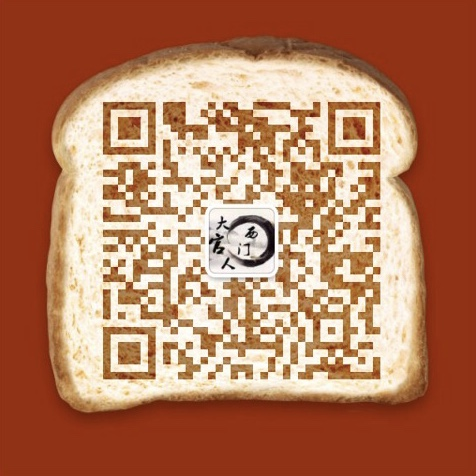
\includegraphics[width=0.3\textwidth]{figs/WeChat.jpg}\\
    \textcolor{gray}{扫码加微信,欢迎技术交流}
\end{center}

% 目录页码使用罗马数字
\pagenumbering{Roman}
\tableofcontents

% 正文使用阿拉伯数字
\clearpage
\pagenumbering{arabic}

\chapter{进阶篇}
鉴于近期事务繁杂,时间精力有限,进阶篇相关内容,请直接参看\href{https://www.freebsd.org/doc/en_US.ISO8859-1/books/handbook/index.html}{官方HandBook}。

\clearpage

%%%%%%%%%%%%%%%%%%%%%%%
\section{zfs文件系统}
%%%%%%%%%%%%%%%%%%%%%%%

%%%%%%%%%%%%%%%%%%%%%%%
\section{ipfw防火墙}
%%%%%%%%%%%%%%%%%%%%%%%

%%%%%%%%%%%%%%%%%%%%%%%
\section{bhyve虚拟机}
%%%%%%%%%%%%%%%%%%%%%%%

%%%%%%%%%%%%%%%%%%%%%%%
\section{jail容器}
%%%%%%%%%%%%%%%%%%%%%%%

%%%%%%%%%%%%%%%%%%%%%%%
\section{安全加固}
%%%%%%%%%%%%%%%%%%%%%%%

% 系统安全等级
% 审计
% 漏洞排查
% 网络参数
%%%%%%%%%%%%%%%%%%%%%%%
\section{深度定制}
%%%%%%%%%%%%%%%%%%%%%%%


\chapter{进阶篇}
鉴于近期事务繁杂,时间精力有限,进阶篇相关内容,请直接参看\href{https://www.freebsd.org/doc/en_US.ISO8859-1/books/handbook/index.html}{官方HandBook}。

\clearpage

%%%%%%%%%%%%%%%%%%%%%%%
\section{zfs文件系统}
%%%%%%%%%%%%%%%%%%%%%%%

%%%%%%%%%%%%%%%%%%%%%%%
\section{ipfw防火墙}
%%%%%%%%%%%%%%%%%%%%%%%

%%%%%%%%%%%%%%%%%%%%%%%
\section{bhyve虚拟机}
%%%%%%%%%%%%%%%%%%%%%%%

%%%%%%%%%%%%%%%%%%%%%%%
\section{jail容器}
%%%%%%%%%%%%%%%%%%%%%%%

%%%%%%%%%%%%%%%%%%%%%%%
\section{安全加固}
%%%%%%%%%%%%%%%%%%%%%%%

% 系统安全等级
% 审计
% 漏洞排查
% 网络参数
%%%%%%%%%%%%%%%%%%%%%%%
\section{深度定制}
%%%%%%%%%%%%%%%%%%%%%%%


\chapter{进阶篇}
鉴于近期事务繁杂,时间精力有限,进阶篇相关内容,请直接参看\href{https://www.freebsd.org/doc/en_US.ISO8859-1/books/handbook/index.html}{官方HandBook}。

\clearpage

%%%%%%%%%%%%%%%%%%%%%%%
\section{zfs文件系统}
%%%%%%%%%%%%%%%%%%%%%%%

%%%%%%%%%%%%%%%%%%%%%%%
\section{ipfw防火墙}
%%%%%%%%%%%%%%%%%%%%%%%

%%%%%%%%%%%%%%%%%%%%%%%
\section{bhyve虚拟机}
%%%%%%%%%%%%%%%%%%%%%%%

%%%%%%%%%%%%%%%%%%%%%%%
\section{jail容器}
%%%%%%%%%%%%%%%%%%%%%%%

%%%%%%%%%%%%%%%%%%%%%%%
\section{安全加固}
%%%%%%%%%%%%%%%%%%%%%%%

% 系统安全等级
% 审计
% 漏洞排查
% 网络参数
%%%%%%%%%%%%%%%%%%%%%%%
\section{深度定制}
%%%%%%%%%%%%%%%%%%%%%%%



%%%%%%%%%%%%%%%%%%%%%%%%%%%%%%%%%
\end{document}
%%%%%%%%%%%%%%%%%%%%%%%%%%%%%%%%%
